\section{Introducción}

\subsection{Motivación y amenazas cuánticas}

Aunque los sistemas satelitales han operado durante décadas bajo el supuesto de que los algoritmos de clave pública clásicos proporcionarían seguridad a largo plazo, la irrupción previsible de computadoras cuánticas de gran escala ha alterado radicalmente ese cálculo. Resulta particularmente llamativo cómo una tecnología que aún se encuentra en etapas de laboratorio ya impone urgencia concreta sobre infraestructuras orbitales que tardan años en diseñarse, lanzarse y mantenerse operativas.

Uno de los desafíos persistentes que surge al analizar constelaciones LEO de próxima generación radica en el modelo de amenaza harvest-now-decrypt-later. Actores con recursos estatales pueden interceptar hoy tráfico encriptado con la expectativa de descifrarlo en cuanto dispongan de capacidad cuántica suficiente. Kim et al. destacan en su revisión sistemática cómo estas restricciones de diseño espacial —limitaciones severas de potencia, memoria volátil y tolerancia a radiación— complican aún más la transición hacia mecanismos de protección poscuántica \cite{Kim2026}. Lejos de ser un problema teórico, la literatura reciente sugiere que varias constelaciones en despliegue activo carecen todavía de una estrategia de migración creíble.

Ghosh y colaboradores, centrados en enfoques lattice-based para enlaces satelitales, subrayan que las características únicas de los canales espacio-tierra (desvanecimiento, retardos variables y anchura de banda asimétrica) exigen soluciones que trasciendan la simple portabilidad de algoritmos terrestres \cite{Ghosh2026}. La convergencia entre mega-constelaciones, comunicaciones 6G-NTN y la computación cuántica no tolera enfoques fragmentarios. Se necesita una resiliencia cuántica sistémica, incorporada desde la capa física hasta los protocolos de red.

\begin{figure}[t]
\centering
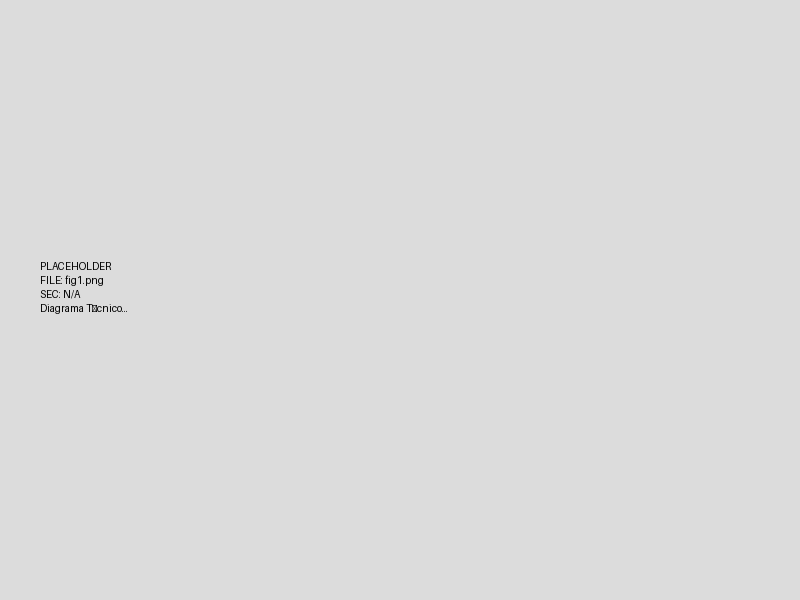
\includegraphics[width=0.92\linewidth]{fig1.png}
\caption{Evolución temporal de amenazas cuánticas contra criptografía clásica en entornos orbitales. Se muestran hitos de desarrollo cuántico, ventanas de vulnerabilidad estimadas y puntos críticos de migración para sistemas satelitales.}
\label{fig:evolucion_amenazas}
\end{figure}

\subsection{Contribuciones principales}

En este trabajo presentamos un marco integral para una infraestructura orbital con resiliencia cuántica. El enfoque combina algoritmos poscuánticos estandarizados por el NIST —en particular ML-KEM, ML-DSA y SLH-DSA— con mecanismos híbridos que preservan compatibilidad hacia atrás mientras habilitan agilidad criptográfica completa \cite{NIST_PQC2024}. 

Nuestro aporte no se limita a la selección de primitivas. Proponemos una arquitectura por capas que considera de forma explícita las restricciones operativas de satélites en órbita baja y media, junto con protocolos de negociación adaptativa y esquemas de gestión de claves distribuidas tolerantes a fallos. Además, entregamos un análisis cuantitativo de overhead en latencia, consumo energético y utilización de ancho de banda obtenido mediante simulaciones de alto fidelidad y emulación en hardware espacial representativo.

Tabla 1 resume las diferencias fundamentales entre enfoques clásicos y poscuánticos bajo condiciones orbitales, destacando métricas que guían las decisiones de diseño del marco propuesto.

\begin{table}[t]
\centering
\caption{Comparación entre criptografía clásica y poscuántica en entornos satelitales}
\label{tab:comparacion_pqc}
\begin{tabular}{lcc}
\hline
\textbf{Aspecto} & \textbf{Clásica (ECC/RSA)} & \textbf{PQC (NIST)} \\
\hline
Tamaño de claves & Pequeño & Significativamente mayor \\
Sobrecarga computacional & Baja & Media-Alta \\
Resistencia a computación cuántica & Nula & Alta \\
Idoneidad para entornos espaciales & Limitada & Requiere optimizaciones \\
\hline
\end{tabular}
\end{table}

\subsection{Organización del documento}

El resto del artículo se estructura de la siguiente manera. La Sección 2 revisa antecedentes y estado del arte, con énfasis en brechas identificadas en implementaciones satelitales. La Sección 3 establece los fundamentos técnicos y restricciones propias de los entornos orbitales. Posteriormente, la Sección 4 detalla el marco propuesto de integración PQC, mientras que la Sección 5 presenta la evaluación de rendimiento y análisis de seguridad. La discusión sobre desafíos prácticos de implementación y estandarización ocupa la Sección 6. Finalmente, la Sección 7 sintetiza conclusiones y delinea líneas de investigación futura.